% !TEX root = ../aas_submission.tex
\documentclass[../main.tex]{subfiles}
\begin{document}

\section{Mathematical description of the poly-line separation measure}
\label{appendix:clustering_maths}

This appendix details the metric used in Section \ref{sec:aggregation_of_volunteer_models} to cluster poly\-lines used by volunteers to model spirals arms. It can be seen as a variant of the Fréchet distance. The metric is illustrated in Figure \ref{fig:spiral_metric_description}.

\begin{figure}
  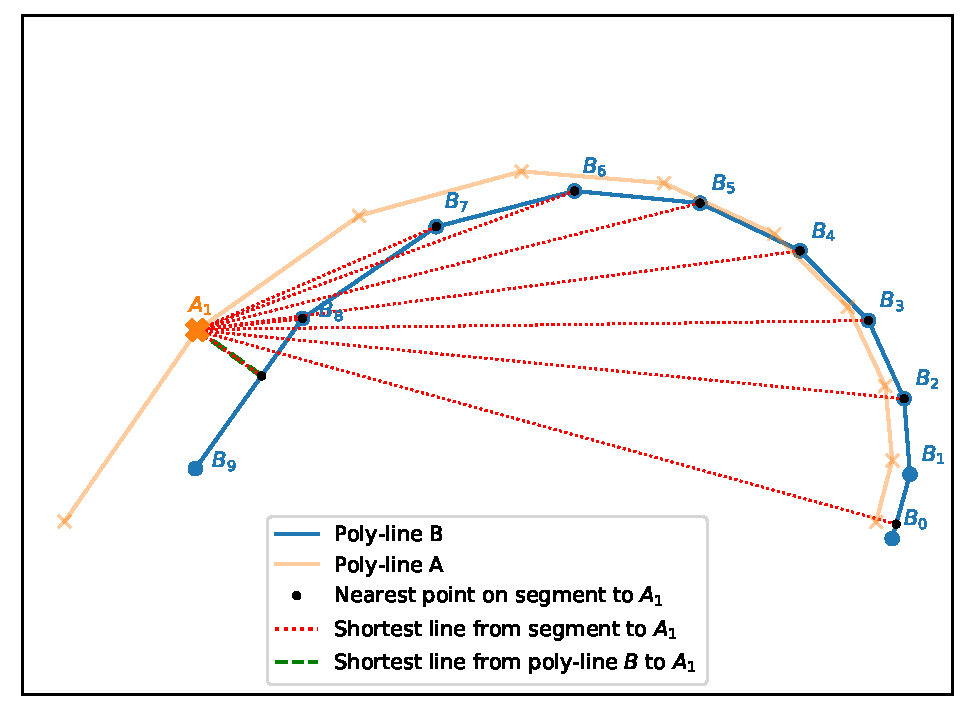
\includegraphics[width=8cm]{images__appendix/spiral_metric_description.pdf}
  \caption{Illustration of the metric used. For each point in line $A$, the shortest distance to each segment in line $B$ is calculated (shown as dotted red lines). The minimum of these distances (corresponding to the line shown in dashed green) is squared.}
  \label{fig:spiral_metric_description}
\end{figure}

First, define a poly-line containing $n$ 2D cartesian coordinates (vertices) as

\begin{equation}
A: \{i \in \mathbb{N};\;i<n\} \longrightarrow \mathbb{R}
^2\end{equation}

We also define a function, $t$, which calculates how far a point $\vec{p}$ is along the line between two other points ($\vec{v}$ and $\vec{w}$):

\begin{equation}
t(\vec{p},\,\vec{v},\,\vec{w}) \equiv \frac{(\vec{p} - \vec{v})\cdot(\vec{v} - \vec{w})}{|\vec{w} - \vec{v}|^2}.
\end{equation}

The minimum distance from $\vec{p}$ to the line segment between $\vec{v}$ and $\vec{w}$ is given by

\begin{equation}
d(\vec{p},\,\vec{v},\,\vec{w}) = \|\left(\vec{v} + \mathrm{min}(\mathrm{max}(t(\vec{p},\,\vec{v},\,\vec{w}),\, 0),\, 1)\;(\vec{w} - \vec{v})\right) - \vec{p}\|
\end{equation}

We then define a ``squared distance'' from the poly-line $A$ (containing $n$ vertices) to the poly-line $B$ (containing $m$ vertices):

\begin{equation}
D(A,\,B) \equiv \frac{1}{n}\sum_{i = 0}^{n} \mathrm{min}\{j \in \mathbb{N}_0,\, j < m;\; d(A_i,\, B_j,\, B_{j+1})^2\}.
\end{equation}

The choice to square the distances and penalize large deviations from other lines was a data-driven choice to improve the results of clustering.

Finally, we define our separation measure between two drawn poly-lines as

\begin{equation}
distance(A,\,B) \equiv D(A,\,B) + D(B,\,A).
\end{equation}


\section{Stacking of multiple SDSS Frames}
\label{appendix:frame_stacking}

 All data required for sigma image creation for stacked frames came from the corrected frames, as detailed in the frame datamodel\footnote{\url{https://data.sdss.org/datamodel/files/BOSS_PHOTOOBJ/frames/RERUN/RUN/CAMCOL/frame.html\#example}}. For each pixel in an SDSS frame, we have

\begin{equation}
\frac{I}{C} = \frac{n}{g} - S + V,
\end{equation}

where $I$ represents the sky-subtracted, corrected image (nanomaggies), $C$ reprents the calibration image, $n$ is the number of electrons captured, $g$ is the gain, $S$ is the Sky value (data units) and $V$ is the dark current, $V = 0 ± \sqrt{v}$ ($v$ being the dark variance).

Given Poisson error,

\begin{equation}
\sigma_n = \sqrt{n}.
\end{equation}

If we stack multiple frames, given $N$ observations of a pixel

\begin{equation}
  \begin{aligned}
n_\mathrm{total} &= \sum_i{n_i} = \sum_i g_i\left(\frac{I_i}{C_i} + S_i - V_i\right),\\
                 &= \sum_{i}\frac{g_i}{C_i}I_i + \sum_i{g_i \left(S_i - V_i\right)} = \sigma_{n_\mathrm{total}}^2.
  \end{aligned}
\end{equation}

This is ideal, and is the level that many fitting software packages work at. As we wish to return to working in units of nanomaggies on a stacked image, further calculation is needed:

\begin{equation}
I = \frac{1}{N}\sum_i I_i,
\end{equation}

\begin{equation}
I = \frac{1}{N}\sum_i C_i\left(\frac{n_i}{g_i} - S_i + V_i\right),
\end{equation}

And so

\begin{equation}
  \sigma_I^2 = \frac{1}{N^2}\sum_i\frac{C_i^2}{g_i^2}\sigma_{n_i}^2 + \frac{1}{N^2}\sum_i C_i^2 \sigma_{S_i}^2 + \frac{1}{N^2}\sum_i C_i^2 \sigma_{V_i}^2.
\end{equation}

We treat the sky value as a constant, such that $\sigma_{S_i}^2 = 0$. Substituting $\sigma_{n_i}^2 = n_i$ as above gives

\begin{equation}
  \sigma_I^2 = \frac{1}{N^2}\sum_i\frac{C_i^2}{g_i^2}n_i + \frac{1}{N^2}\sum_i C_i^2 v_i.
\end{equation}

\begin{equation}
  \sigma_I = \frac{1}{N}\sqrt{\sum_i C_i^2\left(\frac{n_i}{g_i^2} + v_i\right)}.
\end{equation}
Note that this is identical to saying

\begin{equation}
\sigma_I^2 = \frac{1}{N^2}\sum_i\sigma_{I_i}^2.
\end{equation}


\section{Model Fitting}
\label{sec:appendix_model_fitting}
Assume Normal priors on component parameters determined from clustering ($\mu_x$, $\mu_y$, $q$, $Re$), with the spread given by the spread in the clustered values. We therefore have that our final log-likelihood (to be maximised) is the sum of the gaussian log-likelihood of the residuals given the pixel uncertainty and the gaussian log-likelihood of the variation in parameters, given their uncertainty.

The model being rendered is the PSF-convolved sum of the separate components and outputs an ($N_x$, $N_y$) image. The disc, bulge and bar are variations on the boxy S\'ersic profile:

\begin{equation}
I_\mathrm{sersic}(\vec{P}) = I_e \exp\left\{-b_n\left[\left(\frac{r\,(\vec{P})}{R_e}\right)^{1/n} - 1\right]\right\}
\end{equation}

where

\begin{equation}
r\,(\vec{P}) = \left|\begin{pmatrix}
\frac{1}{q} & 0 \\
0 & 1
\end{pmatrix}\begin{pmatrix}
\cos\psi & -\sin\psi\\
\sin\psi & \cos\psi
\end{pmatrix}\left(\vec\mu - \vec{P}\right)\right|_{\ c}.
\end{equation}

The disc is resticted to $n=1; c=2$, bulge to $n\in(0.5, 6); c=2$ and bar to $n\in(0.5, 6); c\in(0.5, 6)$.

The S\'ersic components are actually rendered at 5x the image resolution, and downsampled using the mean pixel brightness. This is a widely used method of approximating the true pixel value, which is an integration over the area of sky inside the pixel. I.e. for a pixel of size $(\delta_x, \delta_y)$

\begin{equation}
I_\mathrm{pix}(\vec{P}) = \frac{1}{\delta_x \delta_y}\int_{-\delta_y/2}^{\delta_y/2}\int_{-\delta_x/2}^{\delta_x/2}\mathrm{d}x\mathrm{d}y\ I_\mathrm{sersic}\left(\vec{P} + \begin{pmatrix}
\delta_x \\
\delta_y \\
\end{pmatrix}\right).
\end{equation}

Spiral arms were restricted to be logarithmic with respect to the inclined, rotated disc. They were rendered in a similar manner to the online interface; using the nearest distance from a pixel to a calculated logarithmic spiral.

An inclined, rotated log spiral requires parameters brightness $I_s$, spread $s$, minimum and maximum $\theta$ ($a$ and $b$), an amplitude $A$, pitch angle $\phi$, position $\vec\mu$, position angle $\psi$ and axis ratio $q$, where $\vec\mu$, $\psi$ and $q$ are inherited from the disc component.

The distance from a pixel to a logarithmic spiral is given by
\begin{equation}
  D_\mathrm{s}(\vec{P}) = \min_{\theta\in[a, b]}\left|\left|\vec{P} - \vec\mu - Ae^{\theta\tan\phi}\begin{pmatrix}
       \cos\psi & \sin\psi\\
       -\sin\psi & \cos\psi
       \end{pmatrix}
       \begin{pmatrix}
       q\cos\theta \\
       \sin\theta \\
       \end{pmatrix}
       \right|\right|^{\ 2}.
\end{equation}

In practise the spiral distance was approximated using the distance to a poly-line with 200 vertices, as solving the above minimization for each pixel at each fitting step is computationally intractable. We also adjust $A$, $a$ and $b$ to account for the rotation of the disc component from its starting value, in order to prevent spirals inadvertendly moving far from starting locations for face-on discs (which have poorly constrained position angles). These adjustments are

\begin{equation}
\begin{aligned}
  A' &= Ae^{\Delta\psi\tan\phi},\\
  a' &= a - \Delta\psi,\\
  b' &= b - \Delta\psi.
\end{aligned}
\end{equation}

The pixel brightness is then calculated as

\begin{equation}
I_\mathrm{spiral}(\vec{P}) = I_\mathrm{disc}(\vec{P}) \times I_s\exp\left(\frac{-D_\mathrm{s}(\vec{P})}{2s^2}\right).
\end{equation}

For the fit, we parametrize disc $I_e$ as the S\'ersic total luminosity, given by

\begin{equation}
L_\mathrm{tot} = I_eR_e^2\ 2\pi n\frac{e^{b_n}}{(b_n)^{2n}}\Gamma(2n).
\end{equation}

Bulge (bar) $I_e$ is reparametrized as ``bulge (bar) fraction'', which we define as

\begin{equation}
F_\mathrm{bulge} = \frac{L_\mathrm{bulge}}{L_\mathrm{disc} + L_\mathrm{bulge}},
\end{equation}

and is limited to be between 0 and 1. Disc luminosity is allowed to take any value greater than or equal to zero.

Similarly, bulge and bar effective radius are reparametrized as their scale relative to the disc ($R_e = R_e / R_{e,\,\mathrm{disc}}$). Bulge and bar are also restricted to have the same poition.


\section{Ancillary Tables}
\begin{table*}
  \centering
  \caption{The maximum, minimum and default values for model parameters. Note that some parameters were allowed to overflow when fitting, for instance an axis ratio greater 1 (signifying a swap of major and minor axis) was allowed, and corrected for once fitting reached completion. This helped avoid the optimizer encountering parameter bounds and failing to converge. Component roll and spiral pitch angle was similarly unconstrained.}
  \begin{tabular}{l|l|r|r|r|r|r}
\hline
Component & Parameter  & Tuning Minimum & Tuning Maximum \\
          &            &  Bound         & Bound          \\
\hline
disc      & $\mu_x$    & -inf           & inf            \\
          & $\mu_y$    & -inf           & inf            \\
          & roll       & -inf           & inf            \\
          & $q$        & 0.25           & 1.2            \\
          & $R_e$      & 0              & inf            \\
          & $\Sigma_e$ & 0              & inf            \\
bulge     & $\mu_x$    & -inf           & inf            \\
          & $\mu_y$    & -inf           & inf            \\
          & roll       & -inf           & inf            \\
          & $q$        & 0.6            & 1.2            \\
          & $R_e / R_\mathrm{disc}$ & 0.01 & 1           \\
          & $(B/T)_r)$ & 0              & 0.99           \\
          & $n$        & 0.5            & 5              \\
bar       & $\mu_x$    & -inf           & inf            \\
          & $\mu_y$    & -inf           & inf            \\
          & roll       & -inf           & inf            \\
          & $q$        & 0.05           & 0.5            \\
          & $R_e / R_\mathrm{disc}$ & 0.05 & 1           \\
          & $(B/T)_r)$ & 0              & 0.99           \\
          & $n$        & 0.3            & 5              \\
          & $c$        & 1              & 6              \\
spiral    & $\Sigma_e$ & 0              & inf            \\
          & spread     & 0              & inf            \\
          & $\phi$     & -85            & 85             \\
\hline
  \centering
  \end{tabular}
  \label{table:bad_values}
\end{table*}

\end{document}
